\section{A Brief Introduction to Online Arithmetic on FPGA}

With the right number representation system, it is possible to perform arithmetic operations MSD first.
Consequently, these online arithmetic operators are attractive for hardware implementation in both serial and parallel forms.
When computing digits serially, they can be chained such that subsequent operations begin before the preceding ones complete.
Parallel implementations tend to be most sensitive to failure in their LSDs, making them more friendly to overclocking than their LSD first counterparts, for which the opposite is true.

In the past, online operators have typically been implemented in binary.
Although Radix-2 modules are the simplest to design and has the shortest cycle time per digit, it has the highest online delay and requires the largest number of cycles to complete calculations~\cite{Tenca1}.
As such, the choice of binary is not absolute.

\subsection{Online Arithmetic}
Traditional arithmetic operators have two common characteristics.
Firstly, their order of operation may be different depending on the operation itself.
A traditional adder, parallel or serial, generates its answers from the LSD to the MSD.
A traditional divider design, on the other hand, generates its answer from the MSD to the LSD~\cite{Brent1}\cite{Srinivas1}.

Due to this inconsistency, arithmetic operators may be forced to compute word-by-word, waiting for all digits to finish in the previous operator before the next can start~\cite{Zhao1}.
Therefore, if a divider follows an adder, the divider has to wait until the adder has completed its computation before it can begin its own.

The other commonality of traditional designs is that their precisions are specified at design-time.
Once built, a 32-bit adder always adds 32 bits together, adding 16-bit numbers usually involves masking the unused bits.
A possible way of making it less inefficient would be using SIMD instructions~\cite{Duncan1}, splitting a large register into a few smaller ones, to execute the same instruction on them in parallel.
This, however, has the tradeoff of being harder to program, and the applications must have sufficient parallelism to exploit.

Online arithmetic does not suffer from the first issue as it performs all arithmetic operations from MSD first~\cite{Ercegovac1}~\cite{Ercegovac2}.
Furthermore, pipelining can be used with online serial arithmetic operators.
Thus the output digit of an earlier operation can be fed into the next operator before the earlier one completes its computation.

\begin{figure}[H]
  \centering
  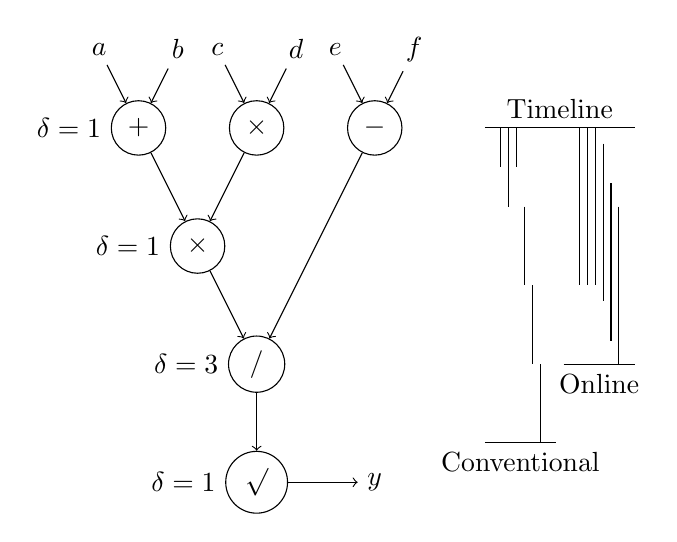
\begin{tikzpicture}
  \path
  (-0.5,5)   node(a) {$a$}
  (0.5,5)    node(b) {$b$}
  (1.0,5)    node(c) {$c$}
  (2,5)      node(d) {$d$}
  (2.5,5)    node(e) {$e$}
  (3.5,5)    node(f) {$f$}

  (0,4)      node[circle,draw,label=left:{$\delta=1$}](p1)  {$+$}
  (1.5,4)    node[circle,draw](p2)                          {$\times$}
  (3,4)      node[circle,draw](p3)                          {$-$}
  (0.75,2.5) node[circle,draw,label=left:{$\delta=1$}](p4)  {$\times$}
  (1.5,1)    node[circle,draw,label=left:{$\delta=3$}](p5)  {$/$}
  (1.5,-0.5) node[circle,draw,label=left:{$\delta=1$}](p6)  {$\surd$}

  (3,-0.5)   node(y) {$y$}
  ;

  \draw[->] (a) -- (p1);
  \draw[->] (b) -- (p1);
  \draw[->] (c) -- (p2);
  \draw[->] (d) -- (p2);
  \draw[->] (e) -- (p3);
  \draw[->] (f) -- (p3);

  \draw[->] (p1) -- (p4);
  \draw[->] (p2) -- (p4);
  \draw[->] (p3) -- (p5);
  \draw[->] (p4) -- (p5);
  \draw[->] (p5) -- (p6);

  \draw[->] (p6) -- (y);

  \draw (4.4,4) -- (6.3,4) node[midway,above]() {Timeline};;
  \draw (4.4,0) -- (5.3,0) node[midway,below]() {Conventional};
  \draw (5.4,1) -- (6.3,1) node[midway,below]() {Online};

  \draw (4.6,4) -- (4.6,3.5);
  \draw (4.7,4) -- (4.7,3);
  \draw (4.8,4) -- (4.8,3.5);
  \draw (4.9,3) -- (4.9,2);
  \draw (5.0,2) -- (5.0,1);
  \draw (5.1,1) -- (5.1,0);

  \draw (5.6,4) -- (5.6,2);
  \draw (5.7,4) -- (5.7,2);
  \draw (5.8,4) -- (5.8,2);
  \draw (5.9,3.8) -- (5.9,1.8);
  \draw (6.0,3.3) -- (6.0,1.3);
  \draw (6.1,3) -- (6.1,1);

\end{tikzpicture}
  \caption{Computing $y=\sqrt{(a+b)cd/(e-f)}$ with serial online operators~\cite{Ercegovac1}}
  \label{Online}
\end{figure}

As illustrated in figure~\ref{Online}, while each individual operation may take longer than its conventional counterpart, online arithmetic can provide a speedup if the operators are chained in serial.
In addition to the tradeoff in time, individual online arithmetic operators also uses more memory.
To perform all computation from the MSD to the LSD, the use of a redundant number system is compulsory.
However, this redundancy also has its advantage in making the operators scalable.
The time required per digit can be made independent of the length of the operands~\cite{Trivedi1}.

A recently proposed architecture allows the precision of online arithmetic to be controlled at runtime~\cite{Zhao1}.
Traditionally, this runtime control was restricted due to the parallel adders present in the multipliers and dividers.
This architecture reuses a fixed-precision adder and stores residues in on-chip RAM.
As such, a single piece of hardware can be used to calculate to any precision, limited only by the size of the on-chip RAM.

The way online arithmetic alleviates the second problem of fixed precision falls out directly from its MSD-first nature.
Suppose the output of a conventional ripple adder is sampled before it has completed its operation.
In this case, the lower digits would have been completed, but the carry would not have reached the higher ones.
This means the error on the result would be significant, as the top bits were still undetermined~\cite{Shi1}.
However, if the output of a parallel online adder is sampled before its completion, the lower bits would be the undetermined ones.
This means the error of the operation would be small.
With overclocking, online arithmetic operators fail gracefully, losing their precision gradually from the lowest bits first.
Thus, it allows for a runtime tradeoff between precision and frequency~\cite{Shi2}.

% REVISIT JD: find better arguments for high radix on FPGA for these two paras
\subsection{High-radix Arithmetic}
Conventional designs of arithmetic operators use binary representations.
The additional concerns of high-radix operators did not provide justifiable improvements as clock speed of processors kept increasing.
In recent years, the clock speed increase effectively ended, and semiconductor dies shrunk to extremely small sizes.
This means the relative processing time available in a clock period increased.
This enabled and drove the desire for accomplishing more per clock cycle, and high-radix arithmetic is one of them.
It has been shown that, high-radix offers power saving and/or reasonable speedups to the arithmetic operations~\cite{Catanzaro1}\cite{Amin1}\cite{Chen1}.

However, the savings are not without trade-offs.
If the radix chosen is not a power of 2, then this trade-off can become unfavourable if the specification requires much I/O and little computation.
This is because overhead of radix conversion would be significant~\cite{Whyte1}.
It is also unwise to use high-radix representations when the numbers are unusually small, thus making the savings offered by the high-radices negligible~\cite{Catanzaro1}.
The radix also cannot be too high, as the time in a clock period is still limited, if there is too many logic gates for the signal to propagate through, it might become the critical path and slow down the overall design.

The construct of FPGAs might make high-radices more attractive than it is on ICs.
As FPGAs contain small fast carry-ripple adders, high-radix adders may be able to exploit them to obtain significant speedups~\cite{Kornerup1}.

\subsection{High-radix Online Arithmetic}
Using high-radix number representations for online arithmetic is a relatively novel concept.
While there has been some research with similar premises~\cite{Lynch1}\cite{Lynch2}, We take a more direct approach with this project by implementing custom operators made for high-radix online arithmetic on an FPGA.
This will provide empirical results on the method, and will hopefully reveal practical insights along the way.

Furthermore, benchmarking this exotic arithmetic system with popular FPGA applications such as neural networks would be interesting, as there is not much precedence for it.
